
%(BEGIN_QUESTION)
% Copyright 2013, Tony R. Kuphaldt, released under the Creative Commons Attribution License (v 1.0)
% This means you may do almost anything with this work of mine, so long as you give me proper credit

Suppose you are asked to configure the instruments in this flow control loop to sense and display process flow over a range of 0 to 180 gallons per minute (GPM), with the loop controller actuating two split-ranged control valves in a complementary sequence.  A ``Scale-with-Parameters'' (SCP) instruction programmed into the Allen-Bradley controller is supposed to take the analog-to-digital converter's raw count value as an input and scale it into units of GPM for the operator to read on a display:

$$\includegraphics[width=15.5cm]{i02082x01.eps}$$

Write the proper range values inside the boxes near each instrument, showing the proper configuration for each instrument needed to achieve the desired result.

\vskip 20pt \vbox{\hrule \hbox{\strut \vrule{} {\bf Suggestions for Socratic discussion} \vrule} \hrule}

\begin{itemize}
\item{} Suppose the controller displayed a flow of 129 GPM when the actual process flow was 135 GPM.  First, identify {\it two} possible locations in this loop for a calibration error that would account for this discrepancy.  Then, assuming only one fault, explain how you could positively determine the location of this calibration error with a single diagnostic test.
\item{} Suppose valve FV-A was 41\% open and FV-B was 59\% open when the controller output displayed 50\%.  First, identify {\it two} possible locations in this loop for a calibration error that would account for this discrepancy.  Then, assuming only one fault, explain how you could positively determine the location of this calibration error with a single diagnostic test.
\end{itemize}

\underbar{file i02082}
%(END_QUESTION)





%(BEGIN_ANSWER)

%\noindent
%{\bf Partial answer:}

%$$\includegraphics[width=15.5cm]{i02082x03.eps}$$

%Hint: every instrument has at least one {\it input} and one {\it output}.  When instruments are connected together to form a ``loop,'' the signals feed from one instrument to the other in a chain, the output signal of one instrument becoming the input signal of the next in the loop.  This means the output and input signals of instruments so connected must match!

$$\includegraphics[width=15.5cm]{i02082x02.eps}$$

A PV measurement error could lie within the transmitter, or within the controller's analog input.  A single current measurement of the transmitter's signal will tell you where the calibration error resides.

\vskip 10pt

A valve positioning error affecting both control valves could lie within the I/P transducer or within the controller's analog output.  A single current measurement of the controller's output signal will tell you where the calibration error resides.


%(END_ANSWER)





%(BEGIN_NOTES)

%$$\includegraphics[width=15.5cm]{i02082x02.eps}$$

%A PV measurement error could lie within the transmitter, or within the controller's analog input.  A single current measurement of the transmitter's signal will tell you where the calibration error resides.

%\vskip 10pt

%A valve positioning error affecting both control valves could lie within the I/P transducer or within the controller's analog output.  A single current measurement of the controller's output signal will tell you where the calibration error resides.












%\vskip 20pt \vbox{\hrule \hbox{\strut \vrule{} {\bf Suggestions for Socratic discussion} \vrule} \hrule}

%\begin{itemize}
%\item{} Explain why it is important for the instruments in a loop to have compatible input/output ranges.  For example, what if the transmitter had a calibrated range of 0 to 180 GPM but the PLC's input was scaled from 0 to 200 GPM?
%\item{} Why do you suppose this system utilizes {\it two} control valves instead of just one?
%\end{itemize}

%INDEX% Basics, transmitter: input and output ranges
%INDEX% Final Control Elements, valve: split ranging

%(END_NOTES)

